% bristolthesis template.tex file
% Best not to fiddle with this much/at all or things might break
% This needs to line up with the contents of bristolthesis.cls and vice versa
%
%
%
%
%

\documentclass[11pt,twoside]{bristolthesis}

%% Packages - these are those which i used for my thesis so might not be specific to yours
\usepackage{graphicx,latexsym}
\usepackage{amsmath}
\usepackage{amssymb}
\usepackage{amsthm}
\usepackage{longtable}
\usepackage{booktabs}
\usepackage{setspace}
\usepackage{siunitx}
% \usepackage{chemarr} %% Useful for one reaction arrow, useless if you're not a chem major
\usepackage[hyphens]{url}
\usepackage{hyperref}
\usepackage{lmodern}
\usepackage{float}
\floatplacement{figure}{H}
\usepackage{rotating}
% \usepackage{times} % other fonts are available like times, bookman, charter, palatino

%% Paramaters for global document
\hypersetup{colorlinks = false}
\renewcommand{\UrlBreaks}{\do\/\do\a\do\b\do\c\do\d\do\e\do\f\do\g\do\h\do\i\do\j\do\k\do\l\do\m\do\n\do\o\do\p\do\q\do\r\do\s\do\t\do\u\do\v\do\w\do\x\do\y\do\z\do\A\do\B\do\C\do\D\do\E\do\F\do\G\do\H\do\I\do\J\do\K\do\L\do\M\do\N\do\O\do\P\do\Q\do\R\do\S\do\T\do\U\do\V\do\W\do\X\do\Y\do\Z\do\0\do\1\do\2\do\3\do\4\do\5\do\6\do\7\do\8\do\9\do\%\do\.\do\-}
\renewcommand{\chapterautorefname}{Chapter}
\usepackage{times} % other fonts are available like times, bookman, charter, palatino
\usepackage{caption}

% Use ref for internal links
\renewcommand{\hyperref}[2][???]{\autoref{#1}}
\def\chapterautorefname{Chapter}
\def\sectionautorefname{Section}
\def\subsectionautorefname{Subsection}
\usepackage{caption}
\captionsetup{width=5in}

% Syntax highlighting #22
%%%

%%% YAML header functions
\title{I made this template based on thesisdown to comply with the University of Bristol regulations}
\author{Thomas Battram}
\date{September 2020}
\university{University of Bristol}
\faculty{Health Sciences}
\school{Bristol Medical School}
\group{MRC Integrative Epidemiology Unit}
\wordcount{}
\degree{Population Health Sciences}
\logo{figure/index/UoBcrest.pdf}
%%%


%%% The document formatting
\makeatletter
\def\maxwidth{ %
  \ifdim\Gin@nat@width>\linewidth
    \linewidth
  \else
    \Gin@nat@width
  \fi
}
\makeatother

\renewcommand{\contentsname}{Table of Contents}

\setlength{\parskip}{14truept}

  \setlength{\parskip}{\baselineskip}
  \usepackage[parfill]{parskip}

\providecommand{\tightlist}{%
  \setlength{\itemsep}{0pt}\setlength{\parskip}{0pt}}

\Acknowledgements{
THIS IS WHERE YOU THANK PEOPLE!!!!!!!!!!!!!!!!!!!!!!!!!!!!!!!!!!!!!!!!!!!!!!!!!!!!!!!!!!!!!!!!!
}

\Declaration{
I declare that the work in this dissertation was carried out in accordance with the requirements of the University's Regulations and Code of Practice for Research Degree Programmes and that it has not been submitted for any other academic award. Except where indicated by specific reference in the text, the work is the candidate's own work. Work done in collaboration with, or with the assistance of, others, is indicated as such. Any views expressed in the dissertation are those of the author.

\bigskip
\bigskip
\bigskip
\bigskip
\bigskip

Signed

\bigskip
\bigskip
\bigskip
\bigskip
\bigskip

Dated
}

\Abstract{
My abstract will go here and it will be a solid abstract. Full of the things that go in abstracts. Such as numbers, acronyms, other words, and lots of punctuation.

It will have multiple paragraphs too!
}

\Abbreviations{
\textbf{EWAS} - epigenome-wide assoctation study
}

	\usepackage{tikz} \usepackage{booktabs} \usepackage{longtable} \usepackage{siunitx} \pagestyle{plain}
	\usepackage{booktabs}
 \usepackage{longtable}
 \usepackage{array}
 \usepackage{multirow}
 \usepackage{wrapfig}
 \usepackage{float}
 \usepackage{colortbl}
 \usepackage{pdflscape}
 \usepackage{tabu}
 \usepackage{threeparttable}
 \usepackage{threeparttablex}
 \usepackage[normalem]{ulem}
 \usepackage{makecell}
 \usepackage{xcolor}


\newlength{\cslhangindent}
\setlength{\cslhangindent}{1.5em}
\newenvironment{cslreferences}%
  {\setlength{\parindent}{0pt}%
  \everypar{\setlength{\hangindent}{\cslhangindent}}\ignorespaces}%
  {\par}


%%% Main document
\spacing{1}
\begin{document}
  \maketitle

\frontmatter % this stuff will be roman-numbered
\pagestyle{empty} % this removes page numbers from the frontmatter
  \begin{abstract}
    My abstract will go here and it will be a solid abstract. Full of the things that go in abstracts. Such as numbers, acronyms, other words, and lots of punctuation.

    It will have multiple paragraphs too!
  \end{abstract}
  \begin{acknowledgements}
    THIS IS WHERE YOU THANK PEOPLE!!!!!!!!!!!!!!!!!!!!!!!!!!!!!!!!!!!!!!!!!!!!!!!!!!!!!!!!!!!!!!!!!
  \end{acknowledgements}
  \begin{declaration}
    I declare that the work in this dissertation was carried out in accordance with the requirements of the University's Regulations and Code of Practice for Research Degree Programmes and that it has not been submitted for any other academic award. Except where indicated by specific reference in the text, the work is the candidate's own work. Work done in collaboration with, or with the assistance of, others, is indicated as such. Any views expressed in the dissertation are those of the author.

    \bigskip
    \bigskip
    \bigskip
    \bigskip
    \bigskip

    Signed

    \bigskip
    \bigskip
    \bigskip
    \bigskip
    \bigskip

    Dated
  \end{declaration}
  \hypersetup{linkcolor=black}
  \setcounter{tocdepth}{3}
  \tableofcontents
  \listoftables
  \listoffigures

\spacing{1.5}
\mainmatter % here the regular arabic numbering starts
\pagestyle{plain}
\hypertarget{preface}{%
\chapter*{Preface}\label{preface}}
\addcontentsline{toc}{chapter}{Preface}

This template is based on (and in many places copied directly from) the Reed College LaTeX template, but hopefully it will provide a nicer interface for those that have never used TeX or LaTeX before. Using \emph{R Markdown} will also allow you to easily keep track of your analyses in \textbf{R} chunks of code, with the resulting plots and output included as well. The hope is this \emph{R Markdown} template gets you in the habit of doing reproducible research, which benefits you long-term as a researcher, but also will greatly help anyone that is trying to reproduce or build onto your results down the road.

Hopefully, you won't have much of a learning period to go through and you will reap the benefits of a nicely formatted thesis. The use of LaTeX in combination with \emph{Markdown} is more consistent than the output of a word processor, much less prone to corruption or crashing, and the resulting file is smaller than a Word file. While you may have never had problems using Word in the past, your thesis is likely going to be about twice as large and complex as anything you've written before, taxing Word's capabilities. After working with \emph{Markdown} and \textbf{R} together for a few weeks, we are confident this will be your reporting style of choice going forward.

\textbf{Why use it?}

\emph{R Markdown} creates a simple and straightforward way to interface with the beauty of LaTeX. Packages have been written in \textbf{R} to work directly with LaTeX to produce nicely formatting tables and paragraphs. In addition to creating a user friendly interface to LaTeX, \emph{R Markdown} also allows you to read in your data, to analyze it and to visualize it using \textbf{R} functions, and also to provide the documentation and commentary on the results of your project. Further, it allows for \textbf{R} results to be passed inline to the commentary of your results. You'll see more on this later.

\textbf{Who should use it?}

Anyone who needs to use data analysis, math, tables, a lot of figures, complex cross-references, or who just cares about the final appearance of their document should use \emph{R Markdown}. Of particular use should be anyone in the sciences, but the user-friendly nature of \emph{Markdown} and its ability to keep track of and easily include figures, automatically generate a table of contents, index, references, table of figures, etc. should make it of great benefit to nearly anyone writing a thesis project.

\textbf{For additional help with bookdown}
Please visit \href{https://bookdown.org/yihui/bookdown/}{the free online bookdown reference guide}.

\hypertarget{introduction}{%
\chapter{Introduction}\label{introduction}}

This thesis focuses on epigenome-wide association studies (EWAS), which assess the association between DNA methylation changes throughout the genome and traits of interest. BLAH BLAH BLAH

\hypertarget{overview-of-thesis-aims}{%
\section{Overview of thesis aims}\label{overview-of-thesis-aims}}

\textbf{BELOW IS TERRIBLE BUT HELPFUL AS IT GIVES STRUCTURE}

EWAS might be an effective study technique to help provide biomarkers for better diagnosis, prognosis and prediction of disease and traits and further it could provide insight into trait aetiology as well as the downstream effects of a trait. However, with the field in it's infancy, there has yet to be a comprehensive look at what information has been gained from EWAS, what information is still to gain from EWAS in it's current state and whether or not the sites identified in EWAS are likely to be causally related to traits.

In Chapter 3 the aim is to produce a database that brings together all the information currently published (as of X-date) together along with new EWAS with full summary statistics. This vast database will then be explored in Chapter 4, giving a detailed picture of what sites throughout the genome have been discovered in EWAS and exploring why they might have been discovered. NEED TO ADD IN HOW!

After exploring the information already gained from EWAS, Chapter 5 explores the amount of information still to gain from EWAS. NEED TO ADD IN HOW!

The database from Chapter 3 will again be used to extract large EWAS datasets for Chapter 6, where potential biological information from these EWAS will be compared to that of GWAS from the same traits. NEED TO ADD IN HOW!

Finally as an initial means of assessing whether DNA methylation might be causally associated with traits of interest, Chapter 7 will aim to use MR to help infer if DNA methylation identified in EWAS of lung cancer are likely to be causing lung cancer.

\hypertarget{methods}{%
\chapter{Methods}\label{methods}}

\hypertarget{the-ewas-catalog-a-database-of-epigenome-wide-association-studies}{%
\chapter{The EWAS Catalog: a database of epigenome-wide association studies}\label{the-ewas-catalog-a-database-of-epigenome-wide-association-studies}}

\hypertarget{abstract}{%
\section{Abstract}\label{abstract}}

Epigenome-wide association studies (EWAS) seek to understand the link between patterns of DNA methylation, the addition of a methyl group to a DNA molectule that may change how the molecule interacts with other cellular factors, at thousands or millions of sites across the genome to various traits and exposures. In recent years, the increase in availability of DNA methylation measures in population-based cohorts and case-control studies has resulted in a dramatic increase in the number of EWAS being performed and published. To make this rich source of molecular data more accessible, a manually curated database has been made containing CpG-trait associations (at P \textless{} 1x10\textsuperscript{-4}) from published EWAS, each assaying over 100,000 CpGs in at least 100 individuals. The database currently contains these associations from over 150 published EWAS as well as full summary statistics for over 180 million association tests of 418 EWAS in the Avon Longitudinal Study of Parents and Children (ALSPAC) and the Gene Expression Omnibus (GEO). It is accompanied by a web-based tool and R package that allow these associations to be easily queried. This database will give researchers the opportunity to quickly and easily query EWAS associations to gain insight into the molecular underpinnings of disaese as well as the impact of traits and exposures on the DNA methylome. The EWAS Catalog is available at: \url{http://www.ewascatalog.org}.

\hypertarget{introduction-1}{%
\section{Introduction}\label{introduction-1}}

Epigenome-wide association studies (EWAS) aim to assess the associations between phenotypes of interest and DNA methylation across the genome (Mill \& Heijmans, 2013; Rakyan, Down, Balding, \& Beck, 2011; Relton \& Davey Smith, 2010). These associations may then be used for disease diagnosis or prediction (Mill \& Heijmans, 2013; Rakyan et al., 2011; Relton \& Davey Smith, 2010). Also, unlike genetic variants, changes in DNA methylation are responsive to the environment and so may be targeted for treatment. EWAS of smoking (Joehanes et al., 2016), body mass index (BMI) (Wahl et al., 2017) and aging (Horvath, 2013) have shown that various exposures are related to large perturbations in DNA methylation across the genome. Furthermore, a paper recently estimated that over 60\% of the total proportion of BMI variation was captured by DNA methylation at about 150 CpG sites (Banos et al., 2018). In recent years, there has been a dramatic increase in the number of EWAS being performed and published due to technological advancements making it possible to measure DNA methylation at hundreds of thousands of CpG sites cheaply and effectively. Giving researchers easy access to EWAS outputs will help them gain insight into the molecular underpinnings of disease as well as the impact of traits and exposures on the DNA methylome. Furthermore, current collections of summary statistics have already proven useful to various fields, for example the GWAS Catalog (Buniello et al., 2019) has been cited over 2000 times in papers contributing to new methods and exploring the genetic architecture of a plethora of traits.

At the time of making the database, to our knowledge, there were no databases that had collected well-curated EWAS on all traits (no just diseases) in an online database accessible to researchers. During production one database fulfilled those metrics: EWAS Atlas (Li et al., 2019). Other databases are available but are limited to certain diseases (e.g.~MethHC (Huang et al., 2015)). The EWAS Atlas provides a simple-to-use website with annotated CpG sites and information on traits. Ideally a database of EWAS results will provide summary statistics, including betas, standard errors and p-values where provided from publications, in an easily accessible manner, this enables researchers to explore various aspects of the published data without having to retrieve the published article. For example, researchers might compare effect estimates between studies in the database or check to see if their results are replicated in another published study. At the time of writing the EWAS atlas platform did not enable users to download effect estimates and standard errors.

Another caveat is that there is currently only published data on the platform, not full summary statistics from EWAS.

The EWAS Catalog aims to improve upon current databases to 1) allow easy and programmatic access to summary statistics for downstream analyses by researchers and 2) provide full summary statistics from a range of EWAS conducted in multiple cohorts. To this end we have produced The EWAS Catalog, a manually curated database of currently published EWAS, \textbf{NUMBER} (originally 378) EWAS performed in the Avon Longitudinal Study of Parents and Children (ALSPAC) (Boyd et al., 2013; Fraser et al., 2013) and \textbf{NUMBER} (originally 40) EWAS performed from data from the Gene Expression Omnibus (GEO) database. The process and data inclusion are summarised in \textbf{FIGURE} (originally Supplementary Figure 1).

In this chapter, Dr James Staley built the original website, Dr Matthew Suderman has been key in development and maintenance of the website and there was a team to help gather and input the data. I helped develop and maintain the website, gather and input the data, run the EWAS within the ALSPAC cohort and on data from the GEO database. The team, led by myself, is continuing to develop and maintain the database. Full acknowledgements to the team can be found on the website: \url{http://www.ewascatalog.org/about/}.

\hypertarget{methods-1}{%
\section{Methods}\label{methods-1}}

\hypertarget{implementation}{%
\subsection{Implementation}\label{implementation}}

The EWAS Catalog web app was built using the Django Python package (\url{https://djangoproject.com}). The data is stored in a combination of MySQL databases and fast random access files (Li, 2011) and can be queried via the web app or the R package (www.github.com/ewascatalog/ewascatalog-r/).

\hypertarget{overview-of-publication-data-extraction}{%
\subsection{Overview of publication data extraction}\label{overview-of-publication-data-extraction}}

To identify publications, periodic literature searches are performed in PubMed using the search terms: ``epigenome-wide'' OR ``epigenome wide'' OR ``EWAS'' OR ``genome-wide AND methylation'' OR ``genome wide AND methylation''.

Our criteria for inclusion of a study into The EWAS Catalog are as follows:
\begin{enumerate}
\def\labelenumi{\arabic{enumi}.}
\tightlist
\item
  The EWAS performed must contain over 100 humans
\item
  The analysis must contain over 100,000 CpG sites
\item
  The DNA methylation data must be genome-wide
\item
  The study must include previously unpublished EWAS summary statistics
\end{enumerate}
CpG-phenotype associations are extracted from studies at P \textless{} 1x10\textsuperscript{-4}. Variables extracted can be found in \textbf{TABLE} (NO ORIGINAL). All these criteria along with the variables extracted are documented on the website (www.ewascatalog.org/documentation). Experimental factor ontology (EFO) terms were mapped to traits to unify representation of these traits. These EFO terms were manually entered after looking up the trait in the European Bioinformatics Institute database (www.ebi.ac.uk/efo).

Based on these criteria, from 3rd July 2019, The EWAS Catalog contained 540,699 associations from 159 studies.

\hypertarget{overview-of-geo-data-extraction}{%
\subsection{Overview of GEO data extraction}\label{overview-of-geo-data-extraction}}

To recruit additional datasets suitable for new EWAS analysis, the geograbi R package (\url{https://github.com/yousefi138/geograbi}) was used to both query GEO for experiments matching The EWAS Catalog inclusion criteria (described above) and extract relevant DNA methylation and phenotype information. The query was performed on 20 March 2019 and identified 148 such experiments with 32,845 samples where DNA methylation and phenotype information could be successfully extracted. From these, the aim was to repeat the analyses performed in the publications linked by PubMed IDs to each GEO record. Thus, I looked up the corresponding full texts for each dataset and identified the main variables of interest. Of the 148 putative GEO studies, only 34 (23\%) contained sufficient information to replicate the original analysis.

\hypertarget{ewas-methods}{%
\subsection{EWAS methods}\label{ewas-methods}}

\hypertarget{avon-longitudinal-study-of-parents-and-children-alspac}{%
\subsubsection{Avon Longitudinal Study of Parents and Children (ALSPAC)}\label{avon-longitudinal-study-of-parents-and-children-alspac}}

EWAS were conducted for \textbf{NUMBER} (originally 378) continuous and binary traits in peripheral blood DNA methylation of ALSPAC mothers in middle age (N = \textbf{NUMBER} (originally 940) ), generated as part of the Accessible Resource for Integrated Epigenomics Studies (ARIES) project (Relton et al., 2015). The traits were extracted from the same time that blood was drawn for DNA methylation assays.

\textbf{ADD IN QC STEPS AND COHORT INFO HERE} (originally in Supplementary Material)

For all traits, linear regression models were fitted with DNA methylation at each site as the outcome and the phenotype as the exposure. DNA methylation was coded as beta values between 0 and 1. For a particular site, a beta value of 0 represents no methylation being detected in all cells measured and a value of 1 represents all cells being methylated at that site. Covariates included age, the top 10 ancestry principal components, and 20 surrogate variables.

\textbf{ADD IN HOW PCS}

\hypertarget{geo-datasets}{%
\subsubsection{GEO datasets}\label{geo-datasets}}

EWAS were performed using 30 datasets, containing 36 traits were extracted from GEO using the geograbi R package (\url{https://github.com/yousefi138/geograbi}).

\textbf{ADD IN QC STEPS HERE} (originally in Supplementary Material)

A list of all the traits with corresponding citations is provided in \textbf{TABLE} (originally Supplementary Table 1).
For all traits, linear regression models were fitted with DNA methylation as the outcome and the phenotype as the exposure as for the ARIES data. Twenty surrogate variables were included as covariates. Other covariates were considered, but surrogate variables only were used for two reasons: 1) to help automate the process and 2) because covariates used in the original EWAS were not included with many of the GEO datasets.

Statistical analyses were conducted in R (Version 3.3.3). The smartsva package (Chen et al., 2017) was used to create surrogate variables and the ewaff R package (\url{https://github.com/perishky/ewaff}) was used to conduct the EWAS, all p-values are two-sided.

\hypertarget{results}{%
\section{Results}\label{results}}

\hypertarget{database-interface-and-use}{%
\subsection{Database interface and use}\label{database-interface-and-use}}

There are two ways to access this large, curated database: through the main website www.ewascatalog.org or by using the R package ``ewascatalog''. The website provides a simple user interface, which resembles that of the GWAS catalog (Buniello et al., 2019), whereby there is a single search bar to explore the database and links to tabs that contain documentation on the contents and how to cite its use (Figure 1). Users may enter a CpG, gene, genome position or trait into the search bar and it will rapidly return detail for relevant EWAS associations, including CpG, trait, sample size, publication and association (effect and P value) (Figure 1). This information along with additional information such as ancestry, outcome, exposure units, and tissue analysed are available for download as a tab-separated value (tsv) text file. Unlike other EWAS databases, we provide the option of downloading summary results for both the user's search and for the entire database.
\begin{figure}

{\centering 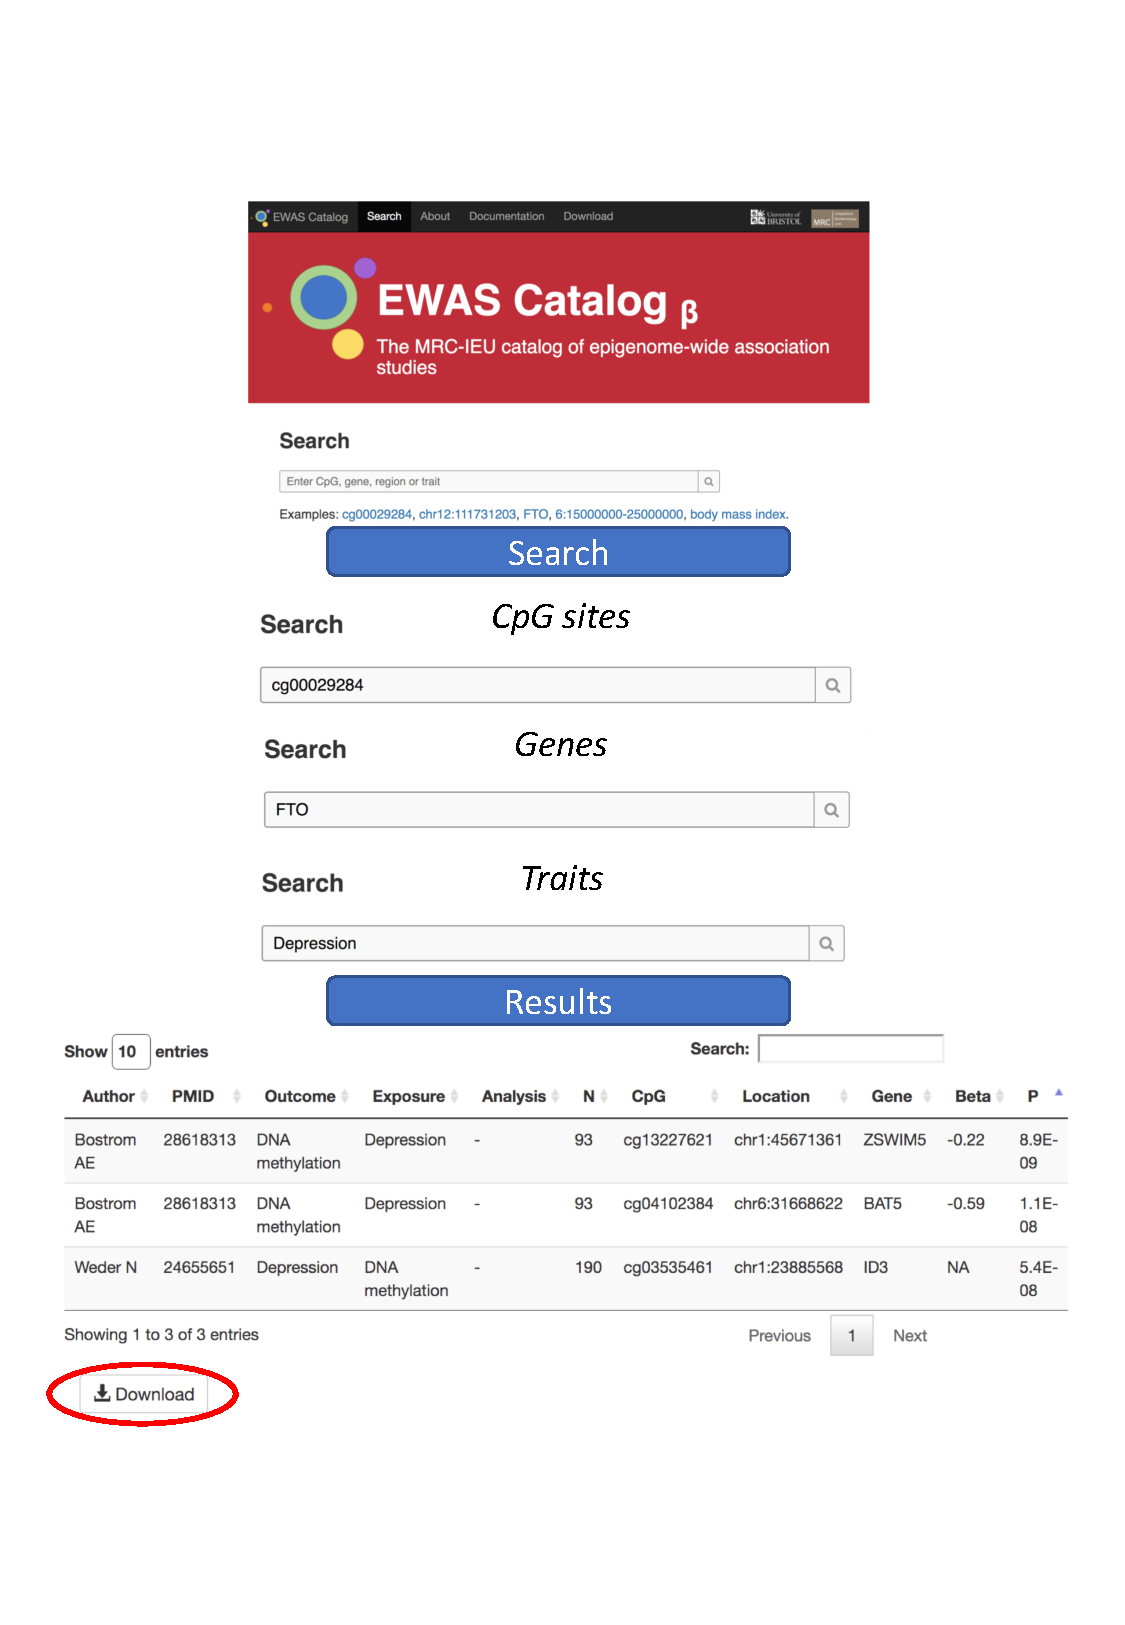
\includegraphics[width=1\linewidth]{/Users/tb13101/Desktop/projects/Main_project/thesis/index/figure/03-ewas_catalog/using_the_catalog} 

}

\caption{Using the EWAS catalog. 
At the top of the figures is the home page URL, ewascatalog.org. 
Below that are examples of three types of searches possible: 
1. CpG sites, 2. genes and 3. traits. 
Finally, the results are displayed after searching the catalog for “Depression”. 
Circled in red is the download button, this button enables the user to download the results of their search as a tab-separated value file. 
This file will contain the information shown on the website as well as additional analysis information.}\label{fig:catalog-use}
\end{figure}
The R package, along with installation instructions and examples are available at \url{https://github.com/ewascatalog/ewascatalog-r/}. Once installed, the database can be queried directly in R using the ``ewascatalog()'' function similar to the website: simply supply the function with a CpG site, gene, genome position or trait and the function returns the same output as is downloadable from the website.

\hypertarget{discussion}{%
\section{Discussion}\label{discussion}}

In this chapter, a database of previously published EWAS and the full summary statistics of 418 newly performed EWAS within ALSPAC and GEO has been established. This is freely available for all researchers to use and provides a platform to explore what information has been gained from EWAS as well as a platform that can be used to pool all existing data to gain new insights into both the EWAS study itself and how DNA methylation associates with traits. Despite the fact The EWAS Atlas has similar aims to The EWAS Catalog, latter provides full summary statistics, extra information and a user-friendly platform to enable more downstream analyses.

The EWAS catalog team will continue to collate and upload newly published EWAS and further increase the number of full summary statistics on the website by performing additional EWAS on available datasets and by inviting EWAS authors to provide full summary statistics. Currently work is ongoing to include additional functionality to allow users to easily and systematically compare their EWAS findings to EWAS in the database. With this full summary data, it is possible to make greater strides into discovering the epigenetic architecture of traits.

Therefore, despite the fact no extra information about EWAS was presented in this chapter, a platform has been made that easily enables us to explore 1) what information has been gained from EWAS and 2) the relationship between DNA methylation and all traits. This will be explored in the next chapters.

\hypertarget{properties-of-ewas}{%
\chapter{Properties of EWAS}\label{properties-of-ewas}}

Here is a reference to Caroline's paper: (Relton \& Davey Smith, 2010)

\hypertarget{m2}{%
\chapter{m2}\label{m2}}

\hypertarget{ewas-gwas-comparison}{%
\chapter{EWAS-GWAS comparison}\label{ewas-gwas-comparison}}

\hypertarget{dnam-lung-cancer-mr}{%
\chapter{DNAm-lung cancer MR}\label{dnam-lung-cancer-mr}}

\hypertarget{conclusion}{%
\chapter*{Conclusion}\label{conclusion}}
\addcontentsline{toc}{chapter}{Conclusion}

If we don't want Conclusion to have a chapter number next to it, we can add the \texttt{\{-\}} attribute.

\textbf{More info}

And here's some other random info: the first paragraph after a chapter title or section head \emph{shouldn't be} indented, because indents are to tell the reader that you're starting a new paragraph. Since that's obvious after a chapter or section title, proper typesetting doesn't add an indent there.

\appendix

\hypertarget{the-first-appendix}{%
\chapter{The First Appendix}\label{the-first-appendix}}

This first appendix includes all of the R chunks of code that were hidden throughout the document (using the \texttt{include\ =\ FALSE} chunk tag) to help with readibility and/or setup.

\textbf{In the main Rmd file}

\textbf{In Chapter \ref{ref-labels}:}

\hypertarget{the-second-appendix-for-fun}{%
\chapter{The Second Appendix, for Fun}\label{the-second-appendix-for-fun}}

\backmatter

\hypertarget{references}{%
\chapter*{References}\label{references}}
\addcontentsline{toc}{chapter}{References}

\markboth{References}{References}

\noindent

\setlength{\parindent}{-0.20in}
\setlength{\leftskip}{0.20in}
\setlength{\parskip}{8pt}

\hypertarget{refs}{}
\begin{cslreferences}
\leavevmode\hypertarget{ref-Banos2018}{}%
Banos, D. T., McCartney, D. L., Battram, T., Hemani, G., Walker, R. M., Morris, S. W., \ldots{} Robinson, M. R. (2018). Bayesian reassessment of the epigenetic architecture of complex traits. \emph{bioRxiv}, 450288. \url{http://doi.org/10.1101/450288}

\leavevmode\hypertarget{ref-Boyd2013}{}%
Boyd, A., Golding, J., Macleod, J., Lawlor, D. A., Fraser, A., Henderson, J., \ldots{} Smith, G. D. (2013). Cohort profile: The 'Children of the 90s'-The index offspring of the avon longitudinal study of parents and children. \emph{International Journal of Epidemiology}, \emph{42}(1), 111--127. \url{http://doi.org/10.1093/ije/dys064}

\leavevmode\hypertarget{ref-Buniello2019}{}%
Buniello, A., Macarthur, J. A. L., Cerezo, M., Harris, L. W., Hayhurst, J., Malangone, C., \ldots{} Parkinson, H. (2019). The NHGRI-EBI GWAS Catalog of published genome-wide association studies, targeted arrays and summary statistics 2019. \emph{Nucleic Acids Research}. \url{http://doi.org/10.1093/nar/gky1120}

\leavevmode\hypertarget{ref-Chen2017}{}%
Chen, J., Behnam, E., Huang, J., Moffatt, M. F., Schaid, D. J., Liang, L., \& Lin, X. (2017). Fast and robust adjustment of cell mixtures in epigenome-wide association studies with SmartSVA. \emph{BMC Genomics}. \url{http://doi.org/10.1186/s12864-017-3808-1}

\leavevmode\hypertarget{ref-Fraser2013}{}%
Fraser, A., Macdonald-wallis, C., Tilling, K., Boyd, A., Golding, J., Davey smith, G., \ldots{} Lawlor, D. A. (2013). Cohort profile: The avon longitudinal study of parents and children: ALSPAC mothers cohort. \emph{International Journal of Epidemiology}. \url{http://doi.org/10.1093/ije/dys066}

\leavevmode\hypertarget{ref-Horvath2013}{}%
Horvath, S. (2013). DNA methylation age of human tissues and cell types. \emph{Genome Biology}, \emph{14}(10), R115. \url{http://doi.org/10.1186/gb-2013-14-10-r115}

\leavevmode\hypertarget{ref-Huang2015}{}%
Huang, W. Y., Hsu, S. D., Huang, H. Y., Sun, Y. M., Chou, C. H., Weng, S. L., \& Huang, H. D. (2015). MethHC: A database of DNA methylation and gene expression in human cancer. \emph{Nucleic Acids Research}. \url{http://doi.org/10.1093/nar/gku1151}

\leavevmode\hypertarget{ref-Joehanes2016}{}%
Joehanes, R., Just, A. C., Marioni, R. E., Pilling, L. C., Reynolds, L. M., Mandaviya, P. R., \ldots{} London, S. J. (2016). Epigenetic Signatures of Cigarette Smoking. \emph{Circulation: Cardiovascular Genetics}, \emph{9}(5), 436--447. \url{http://doi.org/10.1161/CIRCGENETICS.116.001506}

\leavevmode\hypertarget{ref-Li2011}{}%
Li, H. (2011). Tabix: Fast retrieval of sequence features from generic TAB-delimited files. \emph{Bioinformatics}. \url{http://doi.org/10.1093/bioinformatics/btq671}

\leavevmode\hypertarget{ref-Li2019}{}%
Li, M., Zou, D., Li, Z., Gao, R., Sang, J., Zhang, Y., \ldots{} Zhang, Z. (2019). EWAS Atlas: A curated knowledgebase of epigenome-wide association studies. \emph{Nucleic Acids Research}. \url{http://doi.org/10.1093/nar/gky1027}

\leavevmode\hypertarget{ref-Mill2013}{}%
Mill, J., \& Heijmans, B. T. (2013). From promises to practical strategies in epigenetic epidemiology. \emph{Nature Reviews Genetics}, \emph{14}(8), 585--594. \url{http://doi.org/10.1038/nrg3405}

\leavevmode\hypertarget{ref-Rakyan2011}{}%
Rakyan, V. K., Down, T. A., Balding, D. J., \& Beck, S. (2011). Epigenome-wide association studies for common human diseases. \emph{Nature Reviews Genetics}, \emph{12}(8), 529--541. \url{http://doi.org/10.1038/nrg3000}

\leavevmode\hypertarget{ref-Relton2010}{}%
Relton, C. L., \& Davey Smith, G. (2010). Epigenetic Epidemiology of Common Complex Disease: Prospects for Prediction, Prevention, and Treatment. \emph{PLoS Medicine}, \emph{7}(10), e1000356. \url{http://doi.org/10.1371/journal.pmed.1000356}

\leavevmode\hypertarget{ref-Relton2015}{}%
Relton, C. L., Gaunt, T., McArdle, W., Ho, K., Duggirala, A., Shihab, H., \ldots{} Davey Smith, G. (2015). Data Resource Profile: Accessible Resource for Integrated Epigenomic Studies (ARIES). \emph{International Journal of Epidemiology}, \emph{44}(4), 1181--1190. Retrieved from \url{http://dx.doi.org/10.1093/ije/dyv072}

\leavevmode\hypertarget{ref-Wahl2017}{}%
Wahl, S., Drong, A., Lehne, B., Loh, M., Scott, W. R., Kunze, S., \ldots{} Chambers, J. C. (2017). Epigenome-wide association study of body mass index, and the adverse outcomes of adiposity. \emph{Nature}, \emph{541}(7635), 81--86. \url{http://doi.org/10.1038/nature20784}
\end{cslreferences}
  \begin{abbreviations}
    \textbf{EWAS} - epigenome-wide assoctation study
  \end{abbreviations}
\end{document}

